\documentclass[twoside]{book}

% Packages required by doxygen
\usepackage{calc}
\usepackage{doxygen}
\usepackage{graphicx}
\usepackage[utf8]{inputenc}
\usepackage{makeidx}
\usepackage{multicol}
\usepackage{multirow}
\usepackage{textcomp}
\usepackage[table]{xcolor}

% Font selection
\usepackage[T1]{fontenc}
\usepackage{mathptmx}
\usepackage[scaled=.90]{helvet}
\usepackage{courier}
\usepackage{amssymb}
\usepackage{sectsty}
\renewcommand{\familydefault}{\sfdefault}
\allsectionsfont{%
  \fontseries{bc}\selectfont%
  \color{darkgray}%
}
\renewcommand{\DoxyLabelFont}{%
  \fontseries{bc}\selectfont%
  \color{darkgray}%
}

% Page & text layout
\usepackage{geometry}
\geometry{%
  a4paper,%
  top=2.5cm,%
  bottom=2.5cm,%
  left=2.5cm,%
  right=2.5cm%
}
\tolerance=750
\hfuzz=15pt
\hbadness=750
\setlength{\emergencystretch}{15pt}
\setlength{\parindent}{0cm}
\setlength{\parskip}{0.2cm}
\makeatletter
\renewcommand{\paragraph}{%
  \@startsection{paragraph}{4}{0ex}{-1.0ex}{1.0ex}{%
    \normalfont\normalsize\bfseries\SS@parafont%
  }%
}
\renewcommand{\subparagraph}{%
  \@startsection{subparagraph}{5}{0ex}{-1.0ex}{1.0ex}{%
    \normalfont\normalsize\bfseries\SS@subparafont%
  }%
}
\makeatother

% Headers & footers
\usepackage{fancyhdr}
\pagestyle{fancyplain}
\fancyhead[LE]{\fancyplain{}{\bfseries\thepage}}
\fancyhead[CE]{\fancyplain{}{}}
\fancyhead[RE]{\fancyplain{}{\bfseries\leftmark}}
\fancyhead[LO]{\fancyplain{}{\bfseries\rightmark}}
\fancyhead[CO]{\fancyplain{}{}}
\fancyhead[RO]{\fancyplain{}{\bfseries\thepage}}
\fancyfoot[LE]{\fancyplain{}{}}
\fancyfoot[CE]{\fancyplain{}{}}
\fancyfoot[RE]{\fancyplain{}{\bfseries\scriptsize Generated on Thu Jan 2 2014 17\-:37\-:42 for A$\ast$ Implementation by Doxygen }}
\fancyfoot[LO]{\fancyplain{}{\bfseries\scriptsize Generated on Thu Jan 2 2014 17\-:37\-:42 for A$\ast$ Implementation by Doxygen }}
\fancyfoot[CO]{\fancyplain{}{}}
\fancyfoot[RO]{\fancyplain{}{}}
\renewcommand{\footrulewidth}{0.4pt}
\renewcommand{\chaptermark}[1]{%
  \markboth{#1}{}%
}
\renewcommand{\sectionmark}[1]{%
  \markright{\thesection\ #1}%
}

% Indices & bibliography
\usepackage{natbib}
\usepackage[titles]{tocloft}
\setcounter{tocdepth}{3}
\setcounter{secnumdepth}{5}
\makeindex

% Hyperlinks (required, but should be loaded last)
\usepackage{ifpdf}
\ifpdf
  \usepackage[pdftex,pagebackref=true]{hyperref}
\else
  \usepackage[ps2pdf,pagebackref=true]{hyperref}
\fi
\hypersetup{%
  colorlinks=true,%
  linkcolor=blue,%
  citecolor=blue,%
  unicode%
}

% Custom commands
\newcommand{\clearemptydoublepage}{%
  \newpage{\pagestyle{empty}\cleardoublepage}%
}


%===== C O N T E N T S =====

\begin{document}

% Titlepage & ToC
\hypersetup{pageanchor=false}
\pagenumbering{roman}
\begin{titlepage}
\vspace*{7cm}
\begin{center}%
{\Large A$\ast$ Implementation }\\
\vspace*{1cm}
{\large Generated by Doxygen 1.8.5}\\
\vspace*{0.5cm}
{\small Thu Jan 2 2014 17:37:42}\\
\end{center}
\end{titlepage}
\clearemptydoublepage
\tableofcontents
\clearemptydoublepage
\pagenumbering{arabic}
\hypersetup{pageanchor=true}

%--- Begin generated contents ---
\chapter{Hierarchical Index}
\section{Class Hierarchy}
This inheritance list is sorted roughly, but not completely, alphabetically\-:\begin{DoxyCompactList}
\item Comparable\begin{DoxyCompactList}
\item \contentsline{section}{a\-\_\-star.\-A\-Star\-Node}{\pageref{classa__star_1_1_a_star_node}}{}
\begin{DoxyCompactList}
\item \contentsline{section}{a\-\_\-star.\-example.\-A\-Star\-Mesh}{\pageref{classa__star_1_1example_1_1_a_star_mesh}}{}
\end{DoxyCompactList}
\end{DoxyCompactList}
\item \contentsline{section}{test.\-core.\-Drawable}{\pageref{interfacetest_1_1core_1_1_drawable}}{}
\begin{DoxyCompactList}
\item \contentsline{section}{a\-\_\-star.\-follow\-\_\-test.\-Follower}{\pageref{classa__star_1_1follow__test_1_1_follower}}{}
\item \contentsline{section}{a\-\_\-star.\-follow\-\_\-test.\-Mover}{\pageref{classa__star_1_1follow__test_1_1_mover}}{}
\end{DoxyCompactList}
\item \contentsline{section}{test.\-core.\-Main}{\pageref{classtest_1_1core_1_1_main}}{}
\item \contentsline{section}{a\-\_\-star.\-example.\-Mesh\-Creator}{\pageref{classa__star_1_1example_1_1_mesh_creator}}{}
\item \contentsline{section}{a\-\_\-star.\-Pathing\-Algorithms}{\pageref{classa__star_1_1_pathing_algorithms}}{}
\item Runnable\begin{DoxyCompactList}
\item \contentsline{section}{test.\-core.\-Test\-Panel}{\pageref{classtest_1_1core_1_1_test_panel}}{}
\end{DoxyCompactList}
\item J\-Panel\begin{DoxyCompactList}
\item \contentsline{section}{test.\-core.\-Test\-Panel}{\pageref{classtest_1_1core_1_1_test_panel}}{}
\end{DoxyCompactList}
\item Mouse\-Listener\begin{DoxyCompactList}
\item \contentsline{section}{test.\-core.\-Test\-Panel}{\pageref{classtest_1_1core_1_1_test_panel}}{}
\end{DoxyCompactList}
\end{DoxyCompactList}

\chapter{Class Index}
\section{Class List}
Here are the classes, structs, unions and interfaces with brief descriptions\-:\begin{DoxyCompactList}
\item\contentsline{section}{\hyperlink{classa__star_1_1example_1_1_a_star_mesh}{a\-\_\-star.\-example.\-A\-Star\-Mesh} }{\pageref{classa__star_1_1example_1_1_a_star_mesh}}{}
\item\contentsline{section}{\hyperlink{classa__star_1_1_a_star_node}{a\-\_\-star.\-A\-Star\-Node} }{\pageref{classa__star_1_1_a_star_node}}{}
\item\contentsline{section}{\hyperlink{interfacetest_1_1core_1_1_drawable}{test.\-core.\-Drawable} }{\pageref{interfacetest_1_1core_1_1_drawable}}{}
\item\contentsline{section}{\hyperlink{classa__star_1_1follow__test_1_1_follower}{a\-\_\-star.\-follow\-\_\-test.\-Follower} }{\pageref{classa__star_1_1follow__test_1_1_follower}}{}
\item\contentsline{section}{\hyperlink{classtest_1_1core_1_1_main}{test.\-core.\-Main} }{\pageref{classtest_1_1core_1_1_main}}{}
\item\contentsline{section}{\hyperlink{classa__star_1_1example_1_1_mesh_creator}{a\-\_\-star.\-example.\-Mesh\-Creator} }{\pageref{classa__star_1_1example_1_1_mesh_creator}}{}
\item\contentsline{section}{\hyperlink{classa__star_1_1follow__test_1_1_mover}{a\-\_\-star.\-follow\-\_\-test.\-Mover} }{\pageref{classa__star_1_1follow__test_1_1_mover}}{}
\item\contentsline{section}{\hyperlink{classa__star_1_1_pathing_algorithms}{a\-\_\-star.\-Pathing\-Algorithms} }{\pageref{classa__star_1_1_pathing_algorithms}}{}
\item\contentsline{section}{\hyperlink{classtest_1_1core_1_1_test_panel}{test.\-core.\-Test\-Panel} }{\pageref{classtest_1_1core_1_1_test_panel}}{}
\end{DoxyCompactList}

\chapter{Class Documentation}
\hypertarget{classa__star_1_1example_1_1_a_star_mesh}{\section{a\-\_\-star.\-example.\-A\-Star\-Mesh Class Reference}
\label{classa__star_1_1example_1_1_a_star_mesh}\index{a\-\_\-star.\-example.\-A\-Star\-Mesh@{a\-\_\-star.\-example.\-A\-Star\-Mesh}}
}
Inheritance diagram for a\-\_\-star.\-example.\-A\-Star\-Mesh\-:\begin{figure}[H]
\begin{center}
\leavevmode
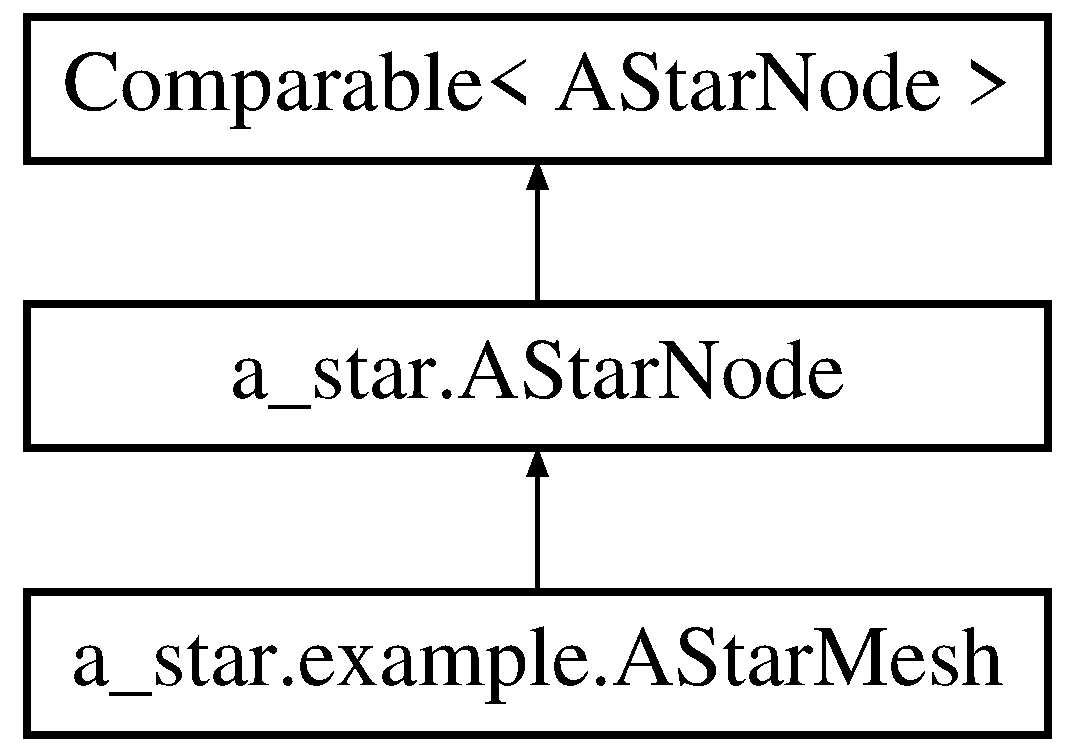
\includegraphics[height=3.000000cm]{classa__star_1_1example_1_1_a_star_mesh}
\end{center}
\end{figure}
\subsection*{Public Member Functions}
\begin{DoxyCompactItemize}
\item 
\hyperlink{classa__star_1_1example_1_1_a_star_mesh_abc6eb8b50c6ab8e853c475d98165e431}{A\-Star\-Mesh} (Array\-List$<$ Point $>$ points)
\item 
void \hyperlink{classa__star_1_1example_1_1_a_star_mesh_ae1fffa184acad06f5764528e39b7315f}{add\-Point} (Point point)
\item 
\hypertarget{classa__star_1_1example_1_1_a_star_mesh_aae4c67360a8ea90a95c9895386c4ed48}{void {\bfseries draw} (Graphics g)}\label{classa__star_1_1example_1_1_a_star_mesh_aae4c67360a8ea90a95c9895386c4ed48}

\item 
\hypertarget{classa__star_1_1example_1_1_a_star_mesh_af87cd72d40a73cadd7bd479e01b79e0e}{void {\bfseries add\-Adjacent} (\hyperlink{classa__star_1_1example_1_1_a_star_mesh}{A\-Star\-Mesh} mesh)}\label{classa__star_1_1example_1_1_a_star_mesh_af87cd72d40a73cadd7bd479e01b79e0e}

\item 
\hypertarget{classa__star_1_1example_1_1_a_star_mesh_a7c329165ace0596ec8780163af782e4e}{boolean {\bfseries equals} (Object o)}\label{classa__star_1_1example_1_1_a_star_mesh_a7c329165ace0596ec8780163af782e4e}

\item 
int \hyperlink{classa__star_1_1example_1_1_a_star_mesh_a3b79dcad4042e9e52bb4def6bf3cd153}{hash\-Code} ()
\item 
float \hyperlink{classa__star_1_1example_1_1_a_star_mesh_a61a6ccb2e73efe277bfa005ae4dc88a9}{calculate\-Move\-Cost} (\hyperlink{classa__star_1_1_a_star_node}{A\-Star\-Node} node)
\item 
Array\-List$<$ \hyperlink{classa__star_1_1_a_star_node}{A\-Star\-Node} $>$ \hyperlink{classa__star_1_1example_1_1_a_star_mesh_a3a5180a2ce88218a07c40d022ab40dc9}{get\-Adjacent\-Nodes} ()
\item 
float \hyperlink{classa__star_1_1example_1_1_a_star_mesh_a75d9ee659d5ce2c72b27c190b5352050}{calculate\-H\-Score} (\hyperlink{classa__star_1_1_a_star_node}{A\-Star\-Node} end)
\item 
\hypertarget{classa__star_1_1example_1_1_a_star_mesh_a7e28f352d55099059192f07d2d34dc54}{void {\bfseries set\-Selected} (boolean selected)}\label{classa__star_1_1example_1_1_a_star_mesh_a7e28f352d55099059192f07d2d34dc54}

\item 
\hypertarget{classa__star_1_1example_1_1_a_star_mesh_a9af6e5662db762cb8c2bdc36d3d824ec}{Point2\-D {\bfseries get\-Center} ()}\label{classa__star_1_1example_1_1_a_star_mesh_a9af6e5662db762cb8c2bdc36d3d824ec}

\end{DoxyCompactItemize}


\subsection{Detailed Description}
An example of a mesh based graph, which implements \hyperlink{classa__star_1_1_a_star_node}{A\-Star\-Node}, and all the abstract methods. This class is more of an example of how to implement A\-Star\-Node.\-java for practical purposes

\begin{DoxyAuthor}{Author}
Nicholas 
\end{DoxyAuthor}


\subsection{Constructor \& Destructor Documentation}
\hypertarget{classa__star_1_1example_1_1_a_star_mesh_abc6eb8b50c6ab8e853c475d98165e431}{\index{a\-\_\-star\-::example\-::\-A\-Star\-Mesh@{a\-\_\-star\-::example\-::\-A\-Star\-Mesh}!A\-Star\-Mesh@{A\-Star\-Mesh}}
\index{A\-Star\-Mesh@{A\-Star\-Mesh}!a_star::example::AStarMesh@{a\-\_\-star\-::example\-::\-A\-Star\-Mesh}}
\subsubsection[{A\-Star\-Mesh}]{\setlength{\rightskip}{0pt plus 5cm}a\-\_\-star.\-example.\-A\-Star\-Mesh.\-A\-Star\-Mesh (
\begin{DoxyParamCaption}
\item[{Array\-List$<$ Point $>$}]{points}
\end{DoxyParamCaption}
)}}\label{classa__star_1_1example_1_1_a_star_mesh_abc6eb8b50c6ab8e853c475d98165e431}
Creates a mesh from the given points/vertices.


\begin{DoxyParams}{Parameters}
{\em points} & An array of vertices \\
\hline
\end{DoxyParams}


\subsection{Member Function Documentation}
\hypertarget{classa__star_1_1example_1_1_a_star_mesh_ae1fffa184acad06f5764528e39b7315f}{\index{a\-\_\-star\-::example\-::\-A\-Star\-Mesh@{a\-\_\-star\-::example\-::\-A\-Star\-Mesh}!add\-Point@{add\-Point}}
\index{add\-Point@{add\-Point}!a_star::example::AStarMesh@{a\-\_\-star\-::example\-::\-A\-Star\-Mesh}}
\subsubsection[{add\-Point}]{\setlength{\rightskip}{0pt plus 5cm}void a\-\_\-star.\-example.\-A\-Star\-Mesh.\-add\-Point (
\begin{DoxyParamCaption}
\item[{Point}]{point}
\end{DoxyParamCaption}
)}}\label{classa__star_1_1example_1_1_a_star_mesh_ae1fffa184acad06f5764528e39b7315f}
Add the point to the list of vertices


\begin{DoxyParams}{Parameters}
{\em point} & \\
\hline
\end{DoxyParams}
\hypertarget{classa__star_1_1example_1_1_a_star_mesh_a75d9ee659d5ce2c72b27c190b5352050}{\index{a\-\_\-star\-::example\-::\-A\-Star\-Mesh@{a\-\_\-star\-::example\-::\-A\-Star\-Mesh}!calculate\-H\-Score@{calculate\-H\-Score}}
\index{calculate\-H\-Score@{calculate\-H\-Score}!a_star::example::AStarMesh@{a\-\_\-star\-::example\-::\-A\-Star\-Mesh}}
\subsubsection[{calculate\-H\-Score}]{\setlength{\rightskip}{0pt plus 5cm}float a\-\_\-star.\-example.\-A\-Star\-Mesh.\-calculate\-H\-Score (
\begin{DoxyParamCaption}
\item[{{\bf A\-Star\-Node}}]{end}
\end{DoxyParamCaption}
)\hspace{0.3cm}{\ttfamily [virtual]}}}\label{classa__star_1_1example_1_1_a_star_mesh_a75d9ee659d5ce2c72b27c190b5352050}
Given the destination node, this method returns a \char`\"{}guess\char`\"{} value of the distance between this node and the end node. This can be the manhatten distance (s.\-x -\/ e.\-x) + (s.\-y -\/ e.\-y) + ... or the as the bird flies distance, so long as it is consistent. Note that this doesn't actually improve pathing, but a better implementation makes the algorithm run faster


\begin{DoxyParams}{Parameters}
{\em end} & the final goal node \\
\hline
\end{DoxyParams}
\begin{DoxyReturn}{Returns}
the guess distance to an end node 
\end{DoxyReturn}


Implements \hyperlink{classa__star_1_1_a_star_node_a64cdac7457076efaf65485371d78b80e}{a\-\_\-star.\-A\-Star\-Node}.

\hypertarget{classa__star_1_1example_1_1_a_star_mesh_a61a6ccb2e73efe277bfa005ae4dc88a9}{\index{a\-\_\-star\-::example\-::\-A\-Star\-Mesh@{a\-\_\-star\-::example\-::\-A\-Star\-Mesh}!calculate\-Move\-Cost@{calculate\-Move\-Cost}}
\index{calculate\-Move\-Cost@{calculate\-Move\-Cost}!a_star::example::AStarMesh@{a\-\_\-star\-::example\-::\-A\-Star\-Mesh}}
\subsubsection[{calculate\-Move\-Cost}]{\setlength{\rightskip}{0pt plus 5cm}float a\-\_\-star.\-example.\-A\-Star\-Mesh.\-calculate\-Move\-Cost (
\begin{DoxyParamCaption}
\item[{{\bf A\-Star\-Node}}]{node}
\end{DoxyParamCaption}
)\hspace{0.3cm}{\ttfamily [virtual]}}}\label{classa__star_1_1example_1_1_a_star_mesh_a61a6ccb2e73efe277bfa005ae4dc88a9}
Given another node, this calculates the cost to move from this node to the given node. This can be done with computing distances, or by factoring in values from terrain features.


\begin{DoxyParams}{Parameters}
{\em node} & the destination node \\
\hline
\end{DoxyParams}
\begin{DoxyReturn}{Returns}
the cost 
\end{DoxyReturn}


Implements \hyperlink{classa__star_1_1_a_star_node_a2b653c71bec99f438a8c9037271bc98a}{a\-\_\-star.\-A\-Star\-Node}.

\hypertarget{classa__star_1_1example_1_1_a_star_mesh_a3a5180a2ce88218a07c40d022ab40dc9}{\index{a\-\_\-star\-::example\-::\-A\-Star\-Mesh@{a\-\_\-star\-::example\-::\-A\-Star\-Mesh}!get\-Adjacent\-Nodes@{get\-Adjacent\-Nodes}}
\index{get\-Adjacent\-Nodes@{get\-Adjacent\-Nodes}!a_star::example::AStarMesh@{a\-\_\-star\-::example\-::\-A\-Star\-Mesh}}
\subsubsection[{get\-Adjacent\-Nodes}]{\setlength{\rightskip}{0pt plus 5cm}Array\-List$<${\bf A\-Star\-Node}$>$ a\-\_\-star.\-example.\-A\-Star\-Mesh.\-get\-Adjacent\-Nodes (
\begin{DoxyParamCaption}
{}
\end{DoxyParamCaption}
)\hspace{0.3cm}{\ttfamily [virtual]}}}\label{classa__star_1_1example_1_1_a_star_mesh_a3a5180a2ce88218a07c40d022ab40dc9}
Returns the nodes that can be traveled to from this node. Note\-: this is basically a directed graph.

\begin{DoxyReturn}{Returns}
A List of nodes that can be traveled to from this node 
\end{DoxyReturn}


Implements \hyperlink{classa__star_1_1_a_star_node_a0472314423f1ff1956f0436f41c77bb6}{a\-\_\-star.\-A\-Star\-Node}.

\hypertarget{classa__star_1_1example_1_1_a_star_mesh_a3b79dcad4042e9e52bb4def6bf3cd153}{\index{a\-\_\-star\-::example\-::\-A\-Star\-Mesh@{a\-\_\-star\-::example\-::\-A\-Star\-Mesh}!hash\-Code@{hash\-Code}}
\index{hash\-Code@{hash\-Code}!a_star::example::AStarMesh@{a\-\_\-star\-::example\-::\-A\-Star\-Mesh}}
\subsubsection[{hash\-Code}]{\setlength{\rightskip}{0pt plus 5cm}int a\-\_\-star.\-example.\-A\-Star\-Mesh.\-hash\-Code (
\begin{DoxyParamCaption}
{}
\end{DoxyParamCaption}
)\hspace{0.3cm}{\ttfamily [virtual]}}}\label{classa__star_1_1example_1_1_a_star_mesh_a3b79dcad4042e9e52bb4def6bf3cd153}
This method must be overridden so that nodes that are equal will return the same hashcode 

Implements \hyperlink{classa__star_1_1_a_star_node_a75c98195daaea78b4bf7c5c058cd792f}{a\-\_\-star.\-A\-Star\-Node}.



The documentation for this class was generated from the following file\-:\begin{DoxyCompactItemize}
\item 
src/a\-\_\-star/example/A\-Star\-Mesh.\-java\end{DoxyCompactItemize}

\hypertarget{classa__star_1_1_a_star_node}{\section{a\-\_\-star.\-A\-Star\-Node Class Reference}
\label{classa__star_1_1_a_star_node}\index{a\-\_\-star.\-A\-Star\-Node@{a\-\_\-star.\-A\-Star\-Node}}
}
Inheritance diagram for a\-\_\-star.\-A\-Star\-Node\-:\begin{figure}[H]
\begin{center}
\leavevmode
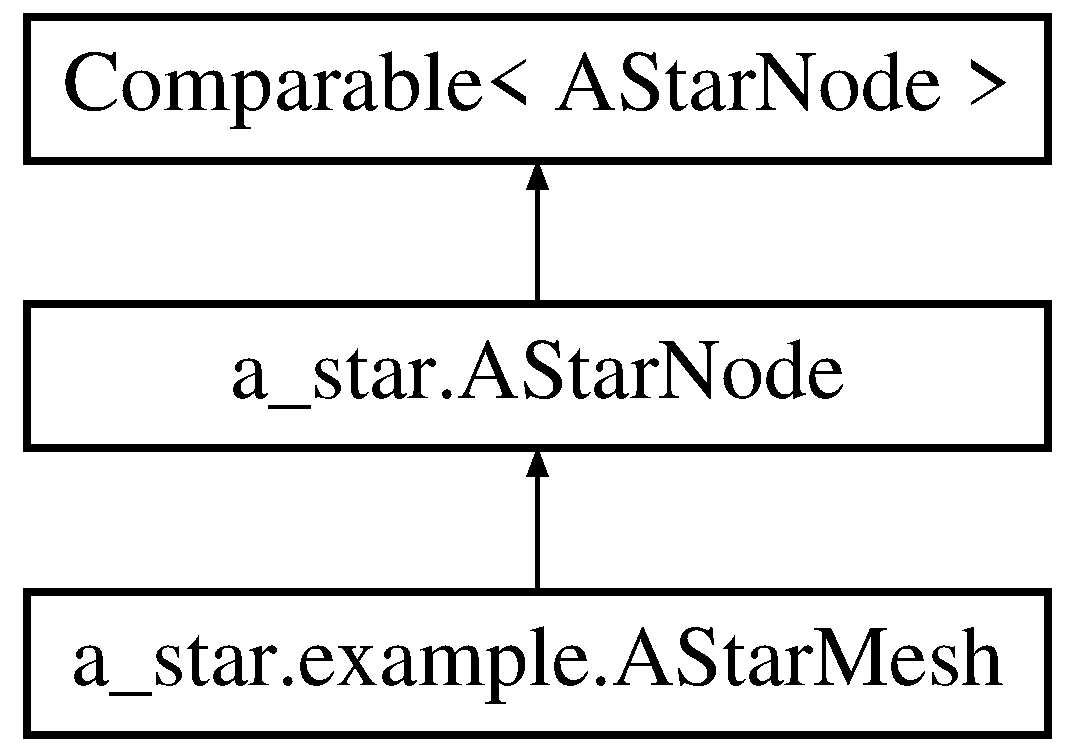
\includegraphics[height=3.000000cm]{classa__star_1_1_a_star_node}
\end{center}
\end{figure}
\subsection*{Public Member Functions}
\begin{DoxyCompactItemize}
\item 
\hypertarget{classa__star_1_1_a_star_node_abf6a3d45b4c9304781df2971f24c72fc}{abstract boolean {\bfseries equals} (Object o)}\label{classa__star_1_1_a_star_node_abf6a3d45b4c9304781df2971f24c72fc}

\item 
abstract int \hyperlink{classa__star_1_1_a_star_node_a75c98195daaea78b4bf7c5c058cd792f}{hash\-Code} ()
\item 
abstract float \hyperlink{classa__star_1_1_a_star_node_a64cdac7457076efaf65485371d78b80e}{calculate\-H\-Score} (\hyperlink{classa__star_1_1_a_star_node}{A\-Star\-Node} end)
\item 
abstract float \hyperlink{classa__star_1_1_a_star_node_a2b653c71bec99f438a8c9037271bc98a}{calculate\-Move\-Cost} (\hyperlink{classa__star_1_1_a_star_node}{A\-Star\-Node} node)
\item 
abstract Iterable$<$ \hyperlink{classa__star_1_1_a_star_node}{A\-Star\-Node} $>$ \hyperlink{classa__star_1_1_a_star_node_a0472314423f1ff1956f0436f41c77bb6}{get\-Adjacent\-Nodes} ()
\item 
\hypertarget{classa__star_1_1_a_star_node_aa1a2db3a747ac0a2676b20984c246d73}{int {\bfseries compare\-To} (\hyperlink{classa__star_1_1_a_star_node}{A\-Star\-Node} node)}\label{classa__star_1_1_a_star_node_aa1a2db3a747ac0a2676b20984c246d73}

\item 
void \hyperlink{classa__star_1_1_a_star_node_a169258256c2ce25e28d7f6c4381869f5}{build\-Path} (Linked\-List$<$ \hyperlink{classa__star_1_1_a_star_node}{A\-Star\-Node} $>$ final\-Path)
\item 
void \hyperlink{classa__star_1_1_a_star_node_adceb6629155eb3ca1f779b9b179b2d2b}{clean} ()
\item 
float \hyperlink{classa__star_1_1_a_star_node_adcf900db191a0ecdf58d0fe1a84ae345}{get\-F\-Score} ()
\item 
float \hyperlink{classa__star_1_1_a_star_node_a285b5d342aee7592cf089218af146d7c}{get\-G\-Score} ()
\item 
void \hyperlink{classa__star_1_1_a_star_node_aedfb508aac1b1aec7626dcacfc87fa54}{set\-G\-Score} (float g\-Score)
\item 
float \hyperlink{classa__star_1_1_a_star_node_ae7d11e89196028b8b664aaac6296c9ee}{get\-H\-Score} ()
\item 
void \hyperlink{classa__star_1_1_a_star_node_a19627a0d4ac73deff6147cb5162fd4d3}{set\-H\-Score} (float h\-Score)
\item 
void \hyperlink{classa__star_1_1_a_star_node_aa3ce3d0f657b61e934e1b1b0a1cf3707}{set\-Parent} (\hyperlink{classa__star_1_1_a_star_node}{A\-Star\-Node} parent)
\end{DoxyCompactItemize}


\subsection{Detailed Description}
This class provides the basic outline for implementing a graph structure, which can be used by the Pathing\-Algorithim.\-java a\-Star\-Path() method. By extending this class an providing correct functionality for the methods, this class will serve as a directed graph capable of finding the shortest path between 2 nodes

\begin{DoxyAuthor}{Author}
Nicholas 
\end{DoxyAuthor}


\subsection{Member Function Documentation}
\hypertarget{classa__star_1_1_a_star_node_a169258256c2ce25e28d7f6c4381869f5}{\index{a\-\_\-star\-::\-A\-Star\-Node@{a\-\_\-star\-::\-A\-Star\-Node}!build\-Path@{build\-Path}}
\index{build\-Path@{build\-Path}!a_star::AStarNode@{a\-\_\-star\-::\-A\-Star\-Node}}
\subsubsection[{build\-Path}]{\setlength{\rightskip}{0pt plus 5cm}void a\-\_\-star.\-A\-Star\-Node.\-build\-Path (
\begin{DoxyParamCaption}
\item[{Linked\-List$<$ {\bf A\-Star\-Node} $>$}]{final\-Path}
\end{DoxyParamCaption}
)}}\label{classa__star_1_1_a_star_node_a169258256c2ce25e28d7f6c4381869f5}
After the shortest path has been calculated, this method puts the nodes into a list by traversing through the parents


\begin{DoxyParams}{Parameters}
{\em final\-Path} & the list to add the path to. \\
\hline
\end{DoxyParams}
\hypertarget{classa__star_1_1_a_star_node_a64cdac7457076efaf65485371d78b80e}{\index{a\-\_\-star\-::\-A\-Star\-Node@{a\-\_\-star\-::\-A\-Star\-Node}!calculate\-H\-Score@{calculate\-H\-Score}}
\index{calculate\-H\-Score@{calculate\-H\-Score}!a_star::AStarNode@{a\-\_\-star\-::\-A\-Star\-Node}}
\subsubsection[{calculate\-H\-Score}]{\setlength{\rightskip}{0pt plus 5cm}abstract float a\-\_\-star.\-A\-Star\-Node.\-calculate\-H\-Score (
\begin{DoxyParamCaption}
\item[{{\bf A\-Star\-Node}}]{end}
\end{DoxyParamCaption}
)\hspace{0.3cm}{\ttfamily [pure virtual]}}}\label{classa__star_1_1_a_star_node_a64cdac7457076efaf65485371d78b80e}
Given the destination node, this method returns a \char`\"{}guess\char`\"{} value of the distance between this node and the end node. This can be the manhatten distance (s.\-x -\/ e.\-x) + (s.\-y -\/ e.\-y) + ... or the as the bird flies distance, so long as it is consistent. Note that this doesn't actually improve pathing, but a better implementation makes the algorithm run faster


\begin{DoxyParams}{Parameters}
{\em end} & the final goal node \\
\hline
\end{DoxyParams}
\begin{DoxyReturn}{Returns}
the guess distance to an end node 
\end{DoxyReturn}


Implemented in \hyperlink{classa__star_1_1example_1_1_a_star_mesh_a75d9ee659d5ce2c72b27c190b5352050}{a\-\_\-star.\-example.\-A\-Star\-Mesh}.

\hypertarget{classa__star_1_1_a_star_node_a2b653c71bec99f438a8c9037271bc98a}{\index{a\-\_\-star\-::\-A\-Star\-Node@{a\-\_\-star\-::\-A\-Star\-Node}!calculate\-Move\-Cost@{calculate\-Move\-Cost}}
\index{calculate\-Move\-Cost@{calculate\-Move\-Cost}!a_star::AStarNode@{a\-\_\-star\-::\-A\-Star\-Node}}
\subsubsection[{calculate\-Move\-Cost}]{\setlength{\rightskip}{0pt plus 5cm}abstract float a\-\_\-star.\-A\-Star\-Node.\-calculate\-Move\-Cost (
\begin{DoxyParamCaption}
\item[{{\bf A\-Star\-Node}}]{node}
\end{DoxyParamCaption}
)\hspace{0.3cm}{\ttfamily [pure virtual]}}}\label{classa__star_1_1_a_star_node_a2b653c71bec99f438a8c9037271bc98a}
Given another node, this calculates the cost to move from this node to the given node. This can be done with computing distances, or by factoring in values from terrain features.


\begin{DoxyParams}{Parameters}
{\em node} & the destination node \\
\hline
\end{DoxyParams}
\begin{DoxyReturn}{Returns}
the cost 
\end{DoxyReturn}


Implemented in \hyperlink{classa__star_1_1example_1_1_a_star_mesh_a61a6ccb2e73efe277bfa005ae4dc88a9}{a\-\_\-star.\-example.\-A\-Star\-Mesh}.

\hypertarget{classa__star_1_1_a_star_node_adceb6629155eb3ca1f779b9b179b2d2b}{\index{a\-\_\-star\-::\-A\-Star\-Node@{a\-\_\-star\-::\-A\-Star\-Node}!clean@{clean}}
\index{clean@{clean}!a_star::AStarNode@{a\-\_\-star\-::\-A\-Star\-Node}}
\subsubsection[{clean}]{\setlength{\rightskip}{0pt plus 5cm}void a\-\_\-star.\-A\-Star\-Node.\-clean (
\begin{DoxyParamCaption}
{}
\end{DoxyParamCaption}
)}}\label{classa__star_1_1_a_star_node_adceb6629155eb3ca1f779b9b179b2d2b}
Cleans up the path nodes after the pathing algorithm has been run. This is automatically called by Pathing\-Algorithm.\-a\-Star\-Path \hypertarget{classa__star_1_1_a_star_node_a0472314423f1ff1956f0436f41c77bb6}{\index{a\-\_\-star\-::\-A\-Star\-Node@{a\-\_\-star\-::\-A\-Star\-Node}!get\-Adjacent\-Nodes@{get\-Adjacent\-Nodes}}
\index{get\-Adjacent\-Nodes@{get\-Adjacent\-Nodes}!a_star::AStarNode@{a\-\_\-star\-::\-A\-Star\-Node}}
\subsubsection[{get\-Adjacent\-Nodes}]{\setlength{\rightskip}{0pt plus 5cm}abstract Iterable$<${\bf A\-Star\-Node}$>$ a\-\_\-star.\-A\-Star\-Node.\-get\-Adjacent\-Nodes (
\begin{DoxyParamCaption}
{}
\end{DoxyParamCaption}
)\hspace{0.3cm}{\ttfamily [pure virtual]}}}\label{classa__star_1_1_a_star_node_a0472314423f1ff1956f0436f41c77bb6}
Returns the nodes that can be traveled to from this node. Note\-: this is basically a directed graph.

\begin{DoxyReturn}{Returns}
A List of nodes that can be traveled to from this node 
\end{DoxyReturn}


Implemented in \hyperlink{classa__star_1_1example_1_1_a_star_mesh_a3a5180a2ce88218a07c40d022ab40dc9}{a\-\_\-star.\-example.\-A\-Star\-Mesh}.

\hypertarget{classa__star_1_1_a_star_node_adcf900db191a0ecdf58d0fe1a84ae345}{\index{a\-\_\-star\-::\-A\-Star\-Node@{a\-\_\-star\-::\-A\-Star\-Node}!get\-F\-Score@{get\-F\-Score}}
\index{get\-F\-Score@{get\-F\-Score}!a_star::AStarNode@{a\-\_\-star\-::\-A\-Star\-Node}}
\subsubsection[{get\-F\-Score}]{\setlength{\rightskip}{0pt plus 5cm}float a\-\_\-star.\-A\-Star\-Node.\-get\-F\-Score (
\begin{DoxyParamCaption}
{}
\end{DoxyParamCaption}
)}}\label{classa__star_1_1_a_star_node_adcf900db191a0ecdf58d0fe1a84ae345}
\begin{DoxyReturn}{Returns}
the f\-Score value (ie g\-Score + h\-Score) 
\end{DoxyReturn}
\hypertarget{classa__star_1_1_a_star_node_a285b5d342aee7592cf089218af146d7c}{\index{a\-\_\-star\-::\-A\-Star\-Node@{a\-\_\-star\-::\-A\-Star\-Node}!get\-G\-Score@{get\-G\-Score}}
\index{get\-G\-Score@{get\-G\-Score}!a_star::AStarNode@{a\-\_\-star\-::\-A\-Star\-Node}}
\subsubsection[{get\-G\-Score}]{\setlength{\rightskip}{0pt plus 5cm}float a\-\_\-star.\-A\-Star\-Node.\-get\-G\-Score (
\begin{DoxyParamCaption}
{}
\end{DoxyParamCaption}
)}}\label{classa__star_1_1_a_star_node_a285b5d342aee7592cf089218af146d7c}
\begin{DoxyReturn}{Returns}
the g\-Score 
\end{DoxyReturn}
\hypertarget{classa__star_1_1_a_star_node_ae7d11e89196028b8b664aaac6296c9ee}{\index{a\-\_\-star\-::\-A\-Star\-Node@{a\-\_\-star\-::\-A\-Star\-Node}!get\-H\-Score@{get\-H\-Score}}
\index{get\-H\-Score@{get\-H\-Score}!a_star::AStarNode@{a\-\_\-star\-::\-A\-Star\-Node}}
\subsubsection[{get\-H\-Score}]{\setlength{\rightskip}{0pt plus 5cm}float a\-\_\-star.\-A\-Star\-Node.\-get\-H\-Score (
\begin{DoxyParamCaption}
{}
\end{DoxyParamCaption}
)}}\label{classa__star_1_1_a_star_node_ae7d11e89196028b8b664aaac6296c9ee}
\begin{DoxyReturn}{Returns}
the h\-Score 
\end{DoxyReturn}
\hypertarget{classa__star_1_1_a_star_node_a75c98195daaea78b4bf7c5c058cd792f}{\index{a\-\_\-star\-::\-A\-Star\-Node@{a\-\_\-star\-::\-A\-Star\-Node}!hash\-Code@{hash\-Code}}
\index{hash\-Code@{hash\-Code}!a_star::AStarNode@{a\-\_\-star\-::\-A\-Star\-Node}}
\subsubsection[{hash\-Code}]{\setlength{\rightskip}{0pt plus 5cm}abstract int a\-\_\-star.\-A\-Star\-Node.\-hash\-Code (
\begin{DoxyParamCaption}
{}
\end{DoxyParamCaption}
)\hspace{0.3cm}{\ttfamily [pure virtual]}}}\label{classa__star_1_1_a_star_node_a75c98195daaea78b4bf7c5c058cd792f}
This method must be overridden so that nodes that are equal will return the same hashcode 

Implemented in \hyperlink{classa__star_1_1example_1_1_a_star_mesh_a3b79dcad4042e9e52bb4def6bf3cd153}{a\-\_\-star.\-example.\-A\-Star\-Mesh}.

\hypertarget{classa__star_1_1_a_star_node_aedfb508aac1b1aec7626dcacfc87fa54}{\index{a\-\_\-star\-::\-A\-Star\-Node@{a\-\_\-star\-::\-A\-Star\-Node}!set\-G\-Score@{set\-G\-Score}}
\index{set\-G\-Score@{set\-G\-Score}!a_star::AStarNode@{a\-\_\-star\-::\-A\-Star\-Node}}
\subsubsection[{set\-G\-Score}]{\setlength{\rightskip}{0pt plus 5cm}void a\-\_\-star.\-A\-Star\-Node.\-set\-G\-Score (
\begin{DoxyParamCaption}
\item[{float}]{g\-Score}
\end{DoxyParamCaption}
)}}\label{classa__star_1_1_a_star_node_aedfb508aac1b1aec7626dcacfc87fa54}

\begin{DoxyParams}{Parameters}
{\em g\-Score} & the g\-Score to set \\
\hline
\end{DoxyParams}
\hypertarget{classa__star_1_1_a_star_node_a19627a0d4ac73deff6147cb5162fd4d3}{\index{a\-\_\-star\-::\-A\-Star\-Node@{a\-\_\-star\-::\-A\-Star\-Node}!set\-H\-Score@{set\-H\-Score}}
\index{set\-H\-Score@{set\-H\-Score}!a_star::AStarNode@{a\-\_\-star\-::\-A\-Star\-Node}}
\subsubsection[{set\-H\-Score}]{\setlength{\rightskip}{0pt plus 5cm}void a\-\_\-star.\-A\-Star\-Node.\-set\-H\-Score (
\begin{DoxyParamCaption}
\item[{float}]{h\-Score}
\end{DoxyParamCaption}
)}}\label{classa__star_1_1_a_star_node_a19627a0d4ac73deff6147cb5162fd4d3}

\begin{DoxyParams}{Parameters}
{\em h\-Score} & the h\-Score to set \\
\hline
\end{DoxyParams}
\hypertarget{classa__star_1_1_a_star_node_aa3ce3d0f657b61e934e1b1b0a1cf3707}{\index{a\-\_\-star\-::\-A\-Star\-Node@{a\-\_\-star\-::\-A\-Star\-Node}!set\-Parent@{set\-Parent}}
\index{set\-Parent@{set\-Parent}!a_star::AStarNode@{a\-\_\-star\-::\-A\-Star\-Node}}
\subsubsection[{set\-Parent}]{\setlength{\rightskip}{0pt plus 5cm}void a\-\_\-star.\-A\-Star\-Node.\-set\-Parent (
\begin{DoxyParamCaption}
\item[{{\bf A\-Star\-Node}}]{parent}
\end{DoxyParamCaption}
)}}\label{classa__star_1_1_a_star_node_aa3ce3d0f657b61e934e1b1b0a1cf3707}
Sets the parent and updates the g\-Score;


\begin{DoxyParams}{Parameters}
{\em parent} & the parent to set \\
\hline
\end{DoxyParams}


The documentation for this class was generated from the following file\-:\begin{DoxyCompactItemize}
\item 
src/a\-\_\-star/A\-Star\-Node.\-java\end{DoxyCompactItemize}

\hypertarget{interfacetest_1_1core_1_1_drawable}{\section{test.\-core.\-Drawable Interface Reference}
\label{interfacetest_1_1core_1_1_drawable}\index{test.\-core.\-Drawable@{test.\-core.\-Drawable}}
}
Inheritance diagram for test.\-core.\-Drawable\-:\begin{figure}[H]
\begin{center}
\leavevmode
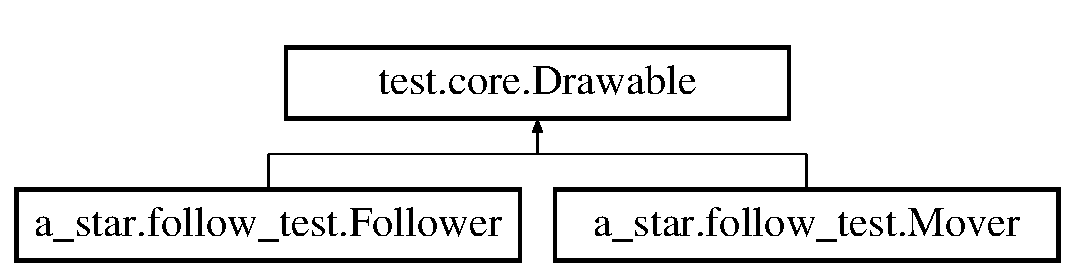
\includegraphics[height=2.000000cm]{interfacetest_1_1core_1_1_drawable}
\end{center}
\end{figure}
\subsection*{Public Member Functions}
\begin{DoxyCompactItemize}
\item 
void \hyperlink{interfacetest_1_1core_1_1_drawable_a98e7fd534ccd6c24dbaaee8bd9fb8e08}{draw} (Graphics g)
\item 
void \hyperlink{interfacetest_1_1core_1_1_drawable_a683aa938b8c5ade02acc08f3bafca3f5}{act} (float time\-Passed)
\end{DoxyCompactItemize}


\subsection{Detailed Description}
Basic interface for drawing/acting test object

\begin{DoxyAuthor}{Author}
Nicholas 
\end{DoxyAuthor}


\subsection{Member Function Documentation}
\hypertarget{interfacetest_1_1core_1_1_drawable_a683aa938b8c5ade02acc08f3bafca3f5}{\index{test\-::core\-::\-Drawable@{test\-::core\-::\-Drawable}!act@{act}}
\index{act@{act}!test::core::Drawable@{test\-::core\-::\-Drawable}}
\subsubsection[{act}]{\setlength{\rightskip}{0pt plus 5cm}void test.\-core.\-Drawable.\-act (
\begin{DoxyParamCaption}
\item[{float}]{time\-Passed}
\end{DoxyParamCaption}
)}}\label{interfacetest_1_1core_1_1_drawable_a683aa938b8c5ade02acc08f3bafca3f5}
Acts the object, using the amount of time\-Passed as a reference


\begin{DoxyParams}{Parameters}
{\em time\-Passed} & \\
\hline
\end{DoxyParams}


Implemented in \hyperlink{classa__star_1_1follow__test_1_1_follower_a2a826175f83c707904cd590e105981b5}{a\-\_\-star.\-follow\-\_\-test.\-Follower}, and \hyperlink{classa__star_1_1follow__test_1_1_mover_a86591ca1d9f386d394fc6f02cac8f15f}{a\-\_\-star.\-follow\-\_\-test.\-Mover}.

\hypertarget{interfacetest_1_1core_1_1_drawable_a98e7fd534ccd6c24dbaaee8bd9fb8e08}{\index{test\-::core\-::\-Drawable@{test\-::core\-::\-Drawable}!draw@{draw}}
\index{draw@{draw}!test::core::Drawable@{test\-::core\-::\-Drawable}}
\subsubsection[{draw}]{\setlength{\rightskip}{0pt plus 5cm}void test.\-core.\-Drawable.\-draw (
\begin{DoxyParamCaption}
\item[{Graphics}]{g}
\end{DoxyParamCaption}
)}}\label{interfacetest_1_1core_1_1_drawable_a98e7fd534ccd6c24dbaaee8bd9fb8e08}
Draws the object to the given graphics


\begin{DoxyParams}{Parameters}
{\em g} & \\
\hline
\end{DoxyParams}


Implemented in \hyperlink{classa__star_1_1follow__test_1_1_follower_a7535656635da25bf0745b16c5ea3b6e1}{a\-\_\-star.\-follow\-\_\-test.\-Follower}, and \hyperlink{classa__star_1_1follow__test_1_1_mover_ac197bf1d7788aeffec0e33dfa745c190}{a\-\_\-star.\-follow\-\_\-test.\-Mover}.



The documentation for this interface was generated from the following file\-:\begin{DoxyCompactItemize}
\item 
src/test/core/Drawable.\-java\end{DoxyCompactItemize}

\hypertarget{classa__star_1_1follow__test_1_1_follower}{\section{a\-\_\-star.\-follow\-\_\-test.\-Follower Class Reference}
\label{classa__star_1_1follow__test_1_1_follower}\index{a\-\_\-star.\-follow\-\_\-test.\-Follower@{a\-\_\-star.\-follow\-\_\-test.\-Follower}}
}
Inheritance diagram for a\-\_\-star.\-follow\-\_\-test.\-Follower\-:\begin{figure}[H]
\begin{center}
\leavevmode
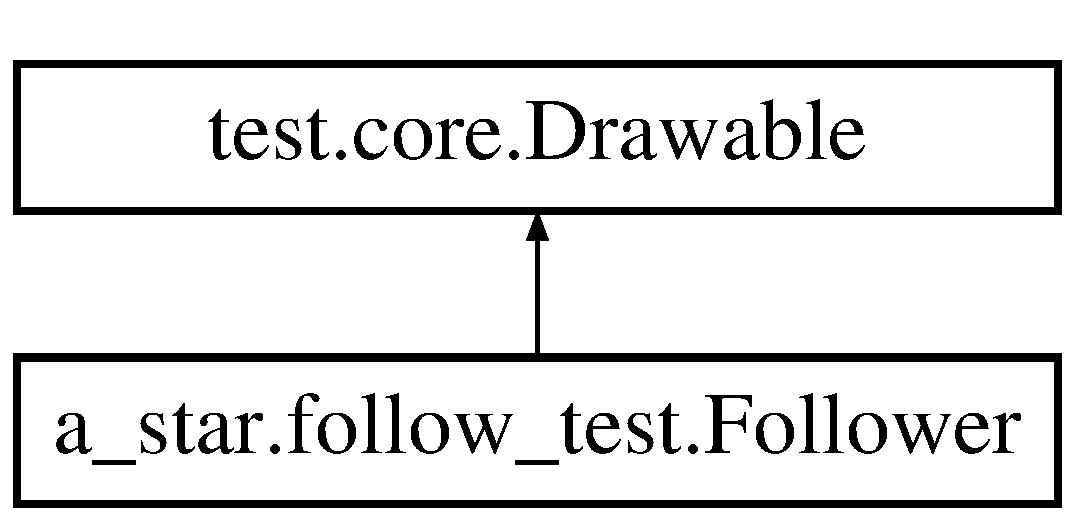
\includegraphics[height=2.000000cm]{classa__star_1_1follow__test_1_1_follower}
\end{center}
\end{figure}
\subsection*{Public Member Functions}
\begin{DoxyCompactItemize}
\item 
\hyperlink{classa__star_1_1follow__test_1_1_follower_a59e6a2777b0e45310baaf5ce428fc711}{Follower} (\hyperlink{classtest_1_1core_1_1_test_panel}{Test\-Panel} main\-Window, Point2\-D start, Array\-List$<$ \hyperlink{classa__star_1_1follow__test_1_1_mover}{Mover} $>$ movers)
\item 
void \hyperlink{classa__star_1_1follow__test_1_1_follower_a7535656635da25bf0745b16c5ea3b6e1}{draw} (Graphics g)
\item 
\hypertarget{classa__star_1_1follow__test_1_1_follower_a923a5bb4c47cc6acf5c310393c611d23}{void {\bfseries clear\-Path} ()}\label{classa__star_1_1follow__test_1_1_follower_a923a5bb4c47cc6acf5c310393c611d23}

\item 
void \hyperlink{classa__star_1_1follow__test_1_1_follower_a2a826175f83c707904cd590e105981b5}{act} (float time\-Passed)
\end{DoxyCompactItemize}


\subsection{Detailed Description}
This class was created to test the path finding of moving object. A \hyperlink{classa__star_1_1follow__test_1_1_follower}{Follower} looks for the closest \hyperlink{classa__star_1_1follow__test_1_1_mover}{Mover} within a given S\-E\-A\-R\-C\-H\-\_\-\-R\-A\-D\-I\-U\-S and if it finds one, it will follow it by continually updating its path

\begin{DoxyAuthor}{Author}
Nicholas 
\end{DoxyAuthor}


\subsection{Constructor \& Destructor Documentation}
\hypertarget{classa__star_1_1follow__test_1_1_follower_a59e6a2777b0e45310baaf5ce428fc711}{\index{a\-\_\-star\-::follow\-\_\-test\-::\-Follower@{a\-\_\-star\-::follow\-\_\-test\-::\-Follower}!Follower@{Follower}}
\index{Follower@{Follower}!a_star::follow_test::Follower@{a\-\_\-star\-::follow\-\_\-test\-::\-Follower}}
\subsubsection[{Follower}]{\setlength{\rightskip}{0pt plus 5cm}a\-\_\-star.\-follow\-\_\-test.\-Follower.\-Follower (
\begin{DoxyParamCaption}
\item[{{\bf Test\-Panel}}]{main\-Window, }
\item[{Point2\-D}]{start, }
\item[{Array\-List$<$ {\bf Mover} $>$}]{movers}
\end{DoxyParamCaption}
)}}\label{classa__star_1_1follow__test_1_1_follower_a59e6a2777b0e45310baaf5ce428fc711}
Creates a follower at the given start position


\begin{DoxyParams}{Parameters}
{\em main\-Window} & reference to the test window \\
\hline
{\em start} & the start location \\
\hline
{\em movers} & a list of all movers \\
\hline
\end{DoxyParams}


\subsection{Member Function Documentation}
\hypertarget{classa__star_1_1follow__test_1_1_follower_a2a826175f83c707904cd590e105981b5}{\index{a\-\_\-star\-::follow\-\_\-test\-::\-Follower@{a\-\_\-star\-::follow\-\_\-test\-::\-Follower}!act@{act}}
\index{act@{act}!a_star::follow_test::Follower@{a\-\_\-star\-::follow\-\_\-test\-::\-Follower}}
\subsubsection[{act}]{\setlength{\rightskip}{0pt plus 5cm}void a\-\_\-star.\-follow\-\_\-test.\-Follower.\-act (
\begin{DoxyParamCaption}
\item[{float}]{time\-Passed}
\end{DoxyParamCaption}
)}}\label{classa__star_1_1follow__test_1_1_follower_a2a826175f83c707904cd590e105981b5}
Acts the object, using the amount of time\-Passed as a reference


\begin{DoxyParams}{Parameters}
{\em time\-Passed} & \\
\hline
\end{DoxyParams}


Implements \hyperlink{interfacetest_1_1core_1_1_drawable_a683aa938b8c5ade02acc08f3bafca3f5}{test.\-core.\-Drawable}.

\hypertarget{classa__star_1_1follow__test_1_1_follower_a7535656635da25bf0745b16c5ea3b6e1}{\index{a\-\_\-star\-::follow\-\_\-test\-::\-Follower@{a\-\_\-star\-::follow\-\_\-test\-::\-Follower}!draw@{draw}}
\index{draw@{draw}!a_star::follow_test::Follower@{a\-\_\-star\-::follow\-\_\-test\-::\-Follower}}
\subsubsection[{draw}]{\setlength{\rightskip}{0pt plus 5cm}void a\-\_\-star.\-follow\-\_\-test.\-Follower.\-draw (
\begin{DoxyParamCaption}
\item[{Graphics}]{g}
\end{DoxyParamCaption}
)}}\label{classa__star_1_1follow__test_1_1_follower_a7535656635da25bf0745b16c5ea3b6e1}
Draws the object to the given graphics


\begin{DoxyParams}{Parameters}
{\em g} & \\
\hline
\end{DoxyParams}


Implements \hyperlink{interfacetest_1_1core_1_1_drawable_a98e7fd534ccd6c24dbaaee8bd9fb8e08}{test.\-core.\-Drawable}.



The documentation for this class was generated from the following file\-:\begin{DoxyCompactItemize}
\item 
src/a\-\_\-star/follow\-\_\-test/Follower.\-java\end{DoxyCompactItemize}

\hypertarget{classtest_1_1core_1_1_main}{\section{test.\-core.\-Main Class Reference}
\label{classtest_1_1core_1_1_main}\index{test.\-core.\-Main@{test.\-core.\-Main}}
}
\subsection*{Static Public Member Functions}
\begin{DoxyCompactItemize}
\item 
\hypertarget{classtest_1_1core_1_1_main_a0a33dc4a053de70be8edc1484bba1475}{static void {\bfseries main} (String\mbox{[}$\,$\mbox{]} args)}\label{classtest_1_1core_1_1_main_a0a33dc4a053de70be8edc1484bba1475}

\end{DoxyCompactItemize}


\subsection{Detailed Description}
Sets up a basic window with a clickable mesh to find the shortest path, and a bunch of movers and followers. Puts the view inside a scroll panel, since it will be large.

\begin{DoxyAuthor}{Author}
Nicholas 
\end{DoxyAuthor}


The documentation for this class was generated from the following file\-:\begin{DoxyCompactItemize}
\item 
src/test/core/Main.\-java\end{DoxyCompactItemize}

\hypertarget{classa__star_1_1example_1_1_mesh_creator}{\section{a\-\_\-star.\-example.\-Mesh\-Creator Class Reference}
\label{classa__star_1_1example_1_1_mesh_creator}\index{a\-\_\-star.\-example.\-Mesh\-Creator@{a\-\_\-star.\-example.\-Mesh\-Creator}}
}
\subsection*{Static Public Member Functions}
\begin{DoxyCompactItemize}
\item 
static \hyperlink{classa__star_1_1example_1_1_a_star_mesh}{A\-Star\-Mesh}\mbox{[}$\,$\mbox{]}\mbox{[}$\,$\mbox{]} \hyperlink{classa__star_1_1example_1_1_mesh_creator_a4e34278d5909159cad43e383c05d1057}{create\-Meshes} (boolean\mbox{[}$\,$\mbox{]}\mbox{[}$\,$\mbox{]} grid)
\item 
\hypertarget{classa__star_1_1example_1_1_mesh_creator_acd2e030759bffe8e4a02074fb2539809}{static boolean\mbox{[}$\,$\mbox{]}\mbox{[}$\,$\mbox{]} {\bfseries test\-Map1} ()}\label{classa__star_1_1example_1_1_mesh_creator_acd2e030759bffe8e4a02074fb2539809}

\item 
static boolean\mbox{[}$\,$\mbox{]}\mbox{[}$\,$\mbox{]} \hyperlink{classa__star_1_1example_1_1_mesh_creator_a6ed3493a725ac4ecb6f60c33023a9ad1}{test\-Map2} ()
\item 
static boolean\mbox{[}$\,$\mbox{]}\mbox{[}$\,$\mbox{]} \hyperlink{classa__star_1_1example_1_1_mesh_creator_a453963a690b84c9d50fe6a9ef8b64fab}{test\-Map3} ()
\end{DoxyCompactItemize}


\subsection{Detailed Description}
This class provides methods to create a grid of meshes to test the pathfinding algorithms. These grids will already set up the graph, by setting adjacent meshes.

\begin{DoxyAuthor}{Author}
Nicholas 
\end{DoxyAuthor}


\subsection{Member Function Documentation}
\hypertarget{classa__star_1_1example_1_1_mesh_creator_a4e34278d5909159cad43e383c05d1057}{\index{a\-\_\-star\-::example\-::\-Mesh\-Creator@{a\-\_\-star\-::example\-::\-Mesh\-Creator}!create\-Meshes@{create\-Meshes}}
\index{create\-Meshes@{create\-Meshes}!a_star::example::MeshCreator@{a\-\_\-star\-::example\-::\-Mesh\-Creator}}
\subsubsection[{create\-Meshes}]{\setlength{\rightskip}{0pt plus 5cm}static {\bf A\-Star\-Mesh} \mbox{[}$\,$\mbox{]}\mbox{[}$\,$\mbox{]} a\-\_\-star.\-example.\-Mesh\-Creator.\-create\-Meshes (
\begin{DoxyParamCaption}
\item[{boolean}]{grid\mbox{[}$\,$\mbox{]}\mbox{[}$\,$\mbox{]}}
\end{DoxyParamCaption}
)\hspace{0.3cm}{\ttfamily [static]}}}\label{classa__star_1_1example_1_1_mesh_creator_a4e34278d5909159cad43e383c05d1057}
Given a grid of booleans, this method builds the connected graph where for any grid\mbox{[}x\mbox{]}\mbox{[}y\mbox{]} == true, a square mesh will be created.


\begin{DoxyParams}{Parameters}
{\em grid} & \\
\hline
\end{DoxyParams}
\begin{DoxyReturn}{Returns}
The grid of \hyperlink{classa__star_1_1example_1_1_a_star_mesh}{A\-Star\-Mesh} connected as a graph structure. 
\end{DoxyReturn}
\hypertarget{classa__star_1_1example_1_1_mesh_creator_a6ed3493a725ac4ecb6f60c33023a9ad1}{\index{a\-\_\-star\-::example\-::\-Mesh\-Creator@{a\-\_\-star\-::example\-::\-Mesh\-Creator}!test\-Map2@{test\-Map2}}
\index{test\-Map2@{test\-Map2}!a_star::example::MeshCreator@{a\-\_\-star\-::example\-::\-Mesh\-Creator}}
\subsubsection[{test\-Map2}]{\setlength{\rightskip}{0pt plus 5cm}static boolean \mbox{[}$\,$\mbox{]}\mbox{[}$\,$\mbox{]} a\-\_\-star.\-example.\-Mesh\-Creator.\-test\-Map2 (
\begin{DoxyParamCaption}
{}
\end{DoxyParamCaption}
)\hspace{0.3cm}{\ttfamily [static]}}}\label{classa__star_1_1example_1_1_mesh_creator_a6ed3493a725ac4ecb6f60c33023a9ad1}
Creates a 200, 100 grid with no holes

\begin{DoxyReturn}{Returns}
matrix of boolean values 
\end{DoxyReturn}
\hypertarget{classa__star_1_1example_1_1_mesh_creator_a453963a690b84c9d50fe6a9ef8b64fab}{\index{a\-\_\-star\-::example\-::\-Mesh\-Creator@{a\-\_\-star\-::example\-::\-Mesh\-Creator}!test\-Map3@{test\-Map3}}
\index{test\-Map3@{test\-Map3}!a_star::example::MeshCreator@{a\-\_\-star\-::example\-::\-Mesh\-Creator}}
\subsubsection[{test\-Map3}]{\setlength{\rightskip}{0pt plus 5cm}static boolean \mbox{[}$\,$\mbox{]}\mbox{[}$\,$\mbox{]} a\-\_\-star.\-example.\-Mesh\-Creator.\-test\-Map3 (
\begin{DoxyParamCaption}
{}
\end{DoxyParamCaption}
)\hspace{0.3cm}{\ttfamily [static]}}}\label{classa__star_1_1example_1_1_mesh_creator_a453963a690b84c9d50fe6a9ef8b64fab}
Creates a 200, 100 grid with random holes

\begin{DoxyReturn}{Returns}
matrix of boolean values 
\end{DoxyReturn}


The documentation for this class was generated from the following file\-:\begin{DoxyCompactItemize}
\item 
src/a\-\_\-star/example/Mesh\-Creator.\-java\end{DoxyCompactItemize}

\hypertarget{classa__star_1_1follow__test_1_1_mover}{\section{a\-\_\-star.\-follow\-\_\-test.\-Mover Class Reference}
\label{classa__star_1_1follow__test_1_1_mover}\index{a\-\_\-star.\-follow\-\_\-test.\-Mover@{a\-\_\-star.\-follow\-\_\-test.\-Mover}}
}
Inheritance diagram for a\-\_\-star.\-follow\-\_\-test.\-Mover\-:\begin{figure}[H]
\begin{center}
\leavevmode
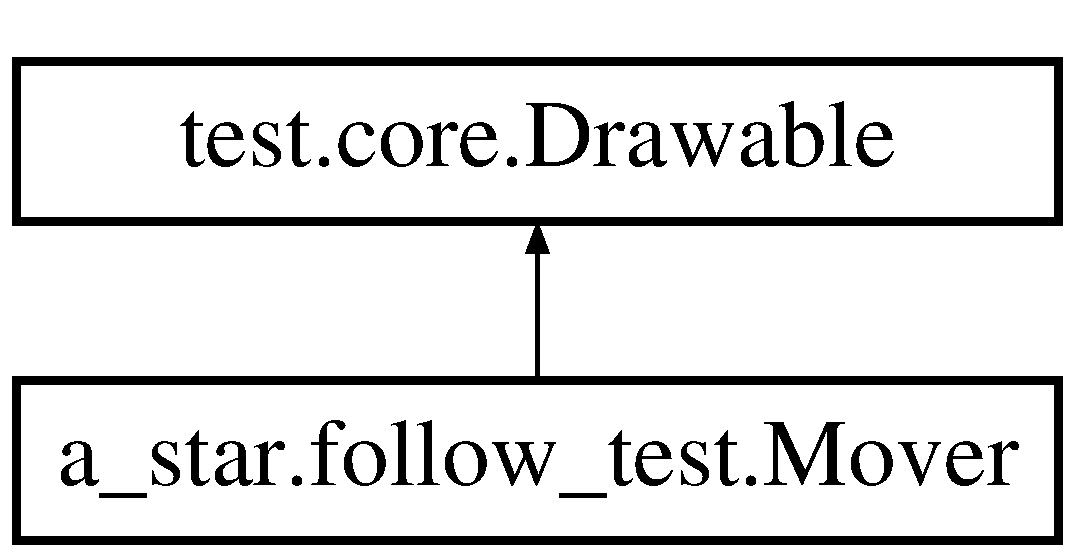
\includegraphics[height=2.000000cm]{classa__star_1_1follow__test_1_1_mover}
\end{center}
\end{figure}
\subsection*{Public Member Functions}
\begin{DoxyCompactItemize}
\item 
\hyperlink{classa__star_1_1follow__test_1_1_mover_a1ccfcf1738bcc78c85f923873e517c0d}{Mover} (\hyperlink{classtest_1_1core_1_1_test_panel}{Test\-Panel} main\-Window, Point2\-D start)
\item 
void \hyperlink{classa__star_1_1follow__test_1_1_mover_ac197bf1d7788aeffec0e33dfa745c190}{draw} (Graphics g)
\item 
void \hyperlink{classa__star_1_1follow__test_1_1_mover_a90243b495db124b15fba9afc79cbcfcf}{clear\-Path} ()
\item 
void \hyperlink{classa__star_1_1follow__test_1_1_mover_a86591ca1d9f386d394fc6f02cac8f15f}{act} (float time\-Passed)
\item 
\hypertarget{classa__star_1_1follow__test_1_1_mover_a16892b4b0ba3f7bd9296bfe1e0b0fd1e}{Point2\-D {\bfseries get\-Location} ()}\label{classa__star_1_1follow__test_1_1_mover_a16892b4b0ba3f7bd9296bfe1e0b0fd1e}

\end{DoxyCompactItemize}


\subsection{Detailed Description}
This class was created to test the path finding of moving object. A \hyperlink{classa__star_1_1follow__test_1_1_mover}{Mover} (if it doesn't have a destination) will calculate a path to a random location and move to it. Movers will be \char`\"{}chased\char`\"{} by Followers if they are close enough

\begin{DoxyAuthor}{Author}
Nicholas 
\end{DoxyAuthor}


\subsection{Constructor \& Destructor Documentation}
\hypertarget{classa__star_1_1follow__test_1_1_mover_a1ccfcf1738bcc78c85f923873e517c0d}{\index{a\-\_\-star\-::follow\-\_\-test\-::\-Mover@{a\-\_\-star\-::follow\-\_\-test\-::\-Mover}!Mover@{Mover}}
\index{Mover@{Mover}!a_star::follow_test::Mover@{a\-\_\-star\-::follow\-\_\-test\-::\-Mover}}
\subsubsection[{Mover}]{\setlength{\rightskip}{0pt plus 5cm}a\-\_\-star.\-follow\-\_\-test.\-Mover.\-Mover (
\begin{DoxyParamCaption}
\item[{{\bf Test\-Panel}}]{main\-Window, }
\item[{Point2\-D}]{start}
\end{DoxyParamCaption}
)}}\label{classa__star_1_1follow__test_1_1_mover_a1ccfcf1738bcc78c85f923873e517c0d}
Creates a mover at the given location


\begin{DoxyParams}{Parameters}
{\em main\-Window} & a reference to the test window \\
\hline
{\em start} & the starting location \\
\hline
\end{DoxyParams}


\subsection{Member Function Documentation}
\hypertarget{classa__star_1_1follow__test_1_1_mover_a86591ca1d9f386d394fc6f02cac8f15f}{\index{a\-\_\-star\-::follow\-\_\-test\-::\-Mover@{a\-\_\-star\-::follow\-\_\-test\-::\-Mover}!act@{act}}
\index{act@{act}!a_star::follow_test::Mover@{a\-\_\-star\-::follow\-\_\-test\-::\-Mover}}
\subsubsection[{act}]{\setlength{\rightskip}{0pt plus 5cm}void a\-\_\-star.\-follow\-\_\-test.\-Mover.\-act (
\begin{DoxyParamCaption}
\item[{float}]{time\-Passed}
\end{DoxyParamCaption}
)}}\label{classa__star_1_1follow__test_1_1_mover_a86591ca1d9f386d394fc6f02cac8f15f}
Acts the object, using the amount of time\-Passed as a reference


\begin{DoxyParams}{Parameters}
{\em time\-Passed} & \\
\hline
\end{DoxyParams}


Implements \hyperlink{interfacetest_1_1core_1_1_drawable_a683aa938b8c5ade02acc08f3bafca3f5}{test.\-core.\-Drawable}.

\hypertarget{classa__star_1_1follow__test_1_1_mover_a90243b495db124b15fba9afc79cbcfcf}{\index{a\-\_\-star\-::follow\-\_\-test\-::\-Mover@{a\-\_\-star\-::follow\-\_\-test\-::\-Mover}!clear\-Path@{clear\-Path}}
\index{clear\-Path@{clear\-Path}!a_star::follow_test::Mover@{a\-\_\-star\-::follow\-\_\-test\-::\-Mover}}
\subsubsection[{clear\-Path}]{\setlength{\rightskip}{0pt plus 5cm}void a\-\_\-star.\-follow\-\_\-test.\-Mover.\-clear\-Path (
\begin{DoxyParamCaption}
{}
\end{DoxyParamCaption}
)}}\label{classa__star_1_1follow__test_1_1_mover_a90243b495db124b15fba9afc79cbcfcf}
Clears the current path that the move is following, it will recalculate a path on the next call to \hyperlink{classa__star_1_1follow__test_1_1_mover_a86591ca1d9f386d394fc6f02cac8f15f}{act()} \hypertarget{classa__star_1_1follow__test_1_1_mover_ac197bf1d7788aeffec0e33dfa745c190}{\index{a\-\_\-star\-::follow\-\_\-test\-::\-Mover@{a\-\_\-star\-::follow\-\_\-test\-::\-Mover}!draw@{draw}}
\index{draw@{draw}!a_star::follow_test::Mover@{a\-\_\-star\-::follow\-\_\-test\-::\-Mover}}
\subsubsection[{draw}]{\setlength{\rightskip}{0pt plus 5cm}void a\-\_\-star.\-follow\-\_\-test.\-Mover.\-draw (
\begin{DoxyParamCaption}
\item[{Graphics}]{g}
\end{DoxyParamCaption}
)}}\label{classa__star_1_1follow__test_1_1_mover_ac197bf1d7788aeffec0e33dfa745c190}
Draws the object to the given graphics


\begin{DoxyParams}{Parameters}
{\em g} & \\
\hline
\end{DoxyParams}


Implements \hyperlink{interfacetest_1_1core_1_1_drawable_a98e7fd534ccd6c24dbaaee8bd9fb8e08}{test.\-core.\-Drawable}.



The documentation for this class was generated from the following file\-:\begin{DoxyCompactItemize}
\item 
src/a\-\_\-star/follow\-\_\-test/Mover.\-java\end{DoxyCompactItemize}

\hypertarget{classa__star_1_1_pathing_algorithms}{\section{a\-\_\-star.\-Pathing\-Algorithms Class Reference}
\label{classa__star_1_1_pathing_algorithms}\index{a\-\_\-star.\-Pathing\-Algorithms@{a\-\_\-star.\-Pathing\-Algorithms}}
}
\subsection*{Static Public Member Functions}
\begin{DoxyCompactItemize}
\item 
static Linked\-List$<$ \hyperlink{classa__star_1_1_a_star_node}{A\-Star\-Node} $>$ \hyperlink{classa__star_1_1_pathing_algorithms_acb3c862843903d83cc1c5faaf81ade91}{a\-Star\-Path} (\hyperlink{classa__star_1_1_a_star_node}{A\-Star\-Node} start, \hyperlink{classa__star_1_1_a_star_node}{A\-Star\-Node} end)
\end{DoxyCompactItemize}


\subsection{Detailed Description}
This class implements the A star pathing algorithm, see the following links for more details \href{http://www.gamedev.net/page/resources/_/technical/artificial-intelligence/a-pathfinding-for-beginners-r2003}{\tt http\-://www.\-gamedev.\-net/page/resources/\-\_\-/technical/artificial-\/intelligence/a-\/pathfinding-\/for-\/beginners-\/r2003} \href{http://en.wikipedia.org/wiki/A}{\tt http\-://en.\-wikipedia.\-org/wiki/\-A}$\ast$\-\_\-search\-\_\-algorithm

\begin{DoxyAuthor}{Author}
Nicholas 
\end{DoxyAuthor}


\subsection{Member Function Documentation}
\hypertarget{classa__star_1_1_pathing_algorithms_acb3c862843903d83cc1c5faaf81ade91}{\index{a\-\_\-star\-::\-Pathing\-Algorithms@{a\-\_\-star\-::\-Pathing\-Algorithms}!a\-Star\-Path@{a\-Star\-Path}}
\index{a\-Star\-Path@{a\-Star\-Path}!a_star::PathingAlgorithms@{a\-\_\-star\-::\-Pathing\-Algorithms}}
\subsubsection[{a\-Star\-Path}]{\setlength{\rightskip}{0pt plus 5cm}static Linked\-List$<${\bf A\-Star\-Node}$>$ a\-\_\-star.\-Pathing\-Algorithms.\-a\-Star\-Path (
\begin{DoxyParamCaption}
\item[{{\bf A\-Star\-Node}}]{start, }
\item[{{\bf A\-Star\-Node}}]{end}
\end{DoxyParamCaption}
)\hspace{0.3cm}{\ttfamily [static]}}}\label{classa__star_1_1_pathing_algorithms_acb3c862843903d83cc1c5faaf81ade91}
This implements the A$\ast$ pathing algorithm to find the shortest path between 2 nodes. If no path exists, this method returns null.

The general overview for the algorithm is as follows\-: there is an open set of nodes that still are available for processing, and a closed set for nodes that have been processed and discarded. Then the algorithm uses the following steps

1, Pop off the node with lowest f score from openset (current), add to closedset
\begin{DoxyEnumerate}
\item If current == end, terminate
\item Else iterate through current's neighbors and if the are not in the closed or open set add to openset, set current as parent if already in openset, if current to neighbor is closer, set parent of neighbor to current
\item Repeat!
\end{DoxyEnumerate}

Currently the implementation uses a hashset for the closedset (optimal) and a hashset for the open set (not optimal). Ideally the open set is a priority queue, however, the queue also needs to be able to handle value updates when the value is already in the queue, which no data structure provided by the Java standard framework provides. In c++ Boosts\-::multi\-\_\-array would be a good fit...


\begin{DoxyParams}{Parameters}
{\em start} & the start node \\
\hline
{\em end} & the end node \\
\hline
\end{DoxyParams}
\begin{DoxyReturn}{Returns}
a Linked\-List of nodes with the final path 
\end{DoxyReturn}


The documentation for this class was generated from the following file\-:\begin{DoxyCompactItemize}
\item 
src/a\-\_\-star/Pathing\-Algorithms.\-java\end{DoxyCompactItemize}

\hypertarget{classtest_1_1core_1_1_test_panel}{\section{test.\-core.\-Test\-Panel Class Reference}
\label{classtest_1_1core_1_1_test_panel}\index{test.\-core.\-Test\-Panel@{test.\-core.\-Test\-Panel}}
}
Inheritance diagram for test.\-core.\-Test\-Panel\-:\begin{figure}[H]
\begin{center}
\leavevmode
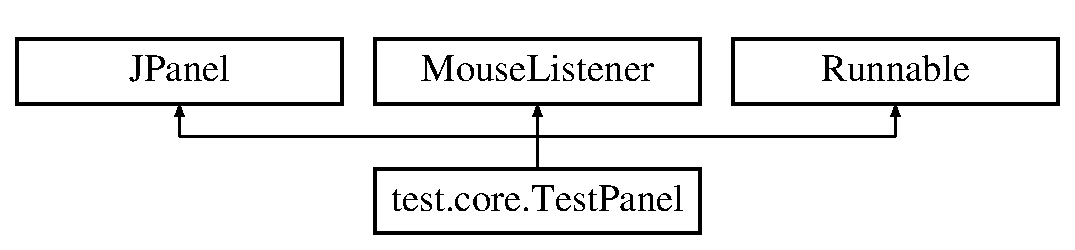
\includegraphics[height=2.000000cm]{classtest_1_1core_1_1_test_panel}
\end{center}
\end{figure}
\subsection*{Public Member Functions}
\begin{DoxyCompactItemize}
\item 
\hyperlink{classtest_1_1core_1_1_test_panel_a800782da9f5f659e10186692b24bcdd4}{Test\-Panel} (\hyperlink{classa__star_1_1example_1_1_a_star_mesh}{A\-Star\-Mesh}\mbox{[}$\,$\mbox{]}\mbox{[}$\,$\mbox{]} mesh\-Grid)
\item 
\hyperlink{classa__star_1_1example_1_1_a_star_mesh}{A\-Star\-Mesh} \hyperlink{classtest_1_1core_1_1_test_panel_a68004836b21a2f98288eb3707e2b5b70}{get\-Mesh\-For\-Point} (Point2\-D point)
\item 
\hypertarget{classtest_1_1core_1_1_test_panel_a5fedf62818cc16c1a6c2cf65af884243}{void {\bfseries paint\-Component} (Graphics g)}\label{classtest_1_1core_1_1_test_panel_a5fedf62818cc16c1a6c2cf65af884243}

\item 
\hypertarget{classtest_1_1core_1_1_test_panel_ad6f7281f40299f2a2dd4ee3f522fdde7}{void {\bfseries mouse\-Clicked} (Mouse\-Event arg0)}\label{classtest_1_1core_1_1_test_panel_ad6f7281f40299f2a2dd4ee3f522fdde7}

\item 
\hypertarget{classtest_1_1core_1_1_test_panel_aba76a7f62f14ca4986e2b644d5dccb6b}{void {\bfseries mouse\-Entered} (Mouse\-Event arg0)}\label{classtest_1_1core_1_1_test_panel_aba76a7f62f14ca4986e2b644d5dccb6b}

\item 
\hypertarget{classtest_1_1core_1_1_test_panel_ac27894fcc70166fdb60eeab851a84e8b}{void {\bfseries mouse\-Exited} (Mouse\-Event arg0)}\label{classtest_1_1core_1_1_test_panel_ac27894fcc70166fdb60eeab851a84e8b}

\item 
\hypertarget{classtest_1_1core_1_1_test_panel_a1ecedb4ae346e2e66b961d01502859d3}{void {\bfseries mouse\-Pressed} (Mouse\-Event arg0)}\label{classtest_1_1core_1_1_test_panel_a1ecedb4ae346e2e66b961d01502859d3}

\item 
\hypertarget{classtest_1_1core_1_1_test_panel_aa95cebcbb7ba1f174411a96aa16d1250}{void {\bfseries mouse\-Released} (Mouse\-Event arg0)}\label{classtest_1_1core_1_1_test_panel_aa95cebcbb7ba1f174411a96aa16d1250}

\item 
\hypertarget{classtest_1_1core_1_1_test_panel_a2031483b4a20bd3ff925d96aa1a3fde9}{void {\bfseries run} ()}\label{classtest_1_1core_1_1_test_panel_a2031483b4a20bd3ff925d96aa1a3fde9}

\item 
\hypertarget{classtest_1_1core_1_1_test_panel_a6a361c0f913c899992460a9213a23a58}{int {\bfseries get\-Width} ()}\label{classtest_1_1core_1_1_test_panel_a6a361c0f913c899992460a9213a23a58}

\item 
\hypertarget{classtest_1_1core_1_1_test_panel_a7fb059c0c6116939d0af03000f8cb82e}{int {\bfseries get\-Height} ()}\label{classtest_1_1core_1_1_test_panel_a7fb059c0c6116939d0af03000f8cb82e}

\end{DoxyCompactItemize}
\subsection*{Static Public Attributes}
\begin{DoxyCompactItemize}
\item 
\hypertarget{classtest_1_1core_1_1_test_panel_a8ca74685e8584cbd65413141cf7f6251}{static final int {\bfseries S\-C\-A\-L\-E} = 12}\label{classtest_1_1core_1_1_test_panel_a8ca74685e8584cbd65413141cf7f6251}

\end{DoxyCompactItemize}


\subsection{Detailed Description}
\hyperlink{classtest_1_1core_1_1_main}{Main} thread for the test view. Controls the general loop (act, render, clear, repeat) as well as interprets user mouse clicks. \begin{DoxyAuthor}{Author}
Nicholas 
\end{DoxyAuthor}


\subsection{Constructor \& Destructor Documentation}
\hypertarget{classtest_1_1core_1_1_test_panel_a800782da9f5f659e10186692b24bcdd4}{\index{test\-::core\-::\-Test\-Panel@{test\-::core\-::\-Test\-Panel}!Test\-Panel@{Test\-Panel}}
\index{Test\-Panel@{Test\-Panel}!test::core::TestPanel@{test\-::core\-::\-Test\-Panel}}
\subsubsection[{Test\-Panel}]{\setlength{\rightskip}{0pt plus 5cm}test.\-core.\-Test\-Panel.\-Test\-Panel (
\begin{DoxyParamCaption}
\item[{{\bf A\-Star\-Mesh}}]{mesh\-Grid\mbox{[}$\,$\mbox{]}\mbox{[}$\,$\mbox{]}}
\end{DoxyParamCaption}
)}}\label{classtest_1_1core_1_1_test_panel_a800782da9f5f659e10186692b24bcdd4}
Creates a J\-Panel with the given graph structure


\begin{DoxyParams}{Parameters}
{\em mesh\-Grid} & \\
\hline
\end{DoxyParams}


\subsection{Member Function Documentation}
\hypertarget{classtest_1_1core_1_1_test_panel_a68004836b21a2f98288eb3707e2b5b70}{\index{test\-::core\-::\-Test\-Panel@{test\-::core\-::\-Test\-Panel}!get\-Mesh\-For\-Point@{get\-Mesh\-For\-Point}}
\index{get\-Mesh\-For\-Point@{get\-Mesh\-For\-Point}!test::core::TestPanel@{test\-::core\-::\-Test\-Panel}}
\subsubsection[{get\-Mesh\-For\-Point}]{\setlength{\rightskip}{0pt plus 5cm}{\bf A\-Star\-Mesh} test.\-core.\-Test\-Panel.\-get\-Mesh\-For\-Point (
\begin{DoxyParamCaption}
\item[{Point2\-D}]{point}
\end{DoxyParamCaption}
)}}\label{classtest_1_1core_1_1_test_panel_a68004836b21a2f98288eb3707e2b5b70}
Given a mouse click point, this method finds the mesh that the click point falls in. Returns null if out of bounds, or no mesh exists


\begin{DoxyParams}{Parameters}
{\em point} & the point within the jpanel \\
\hline
\end{DoxyParams}
\begin{DoxyReturn}{Returns}
A\-Star\-Mesh for that is at that point 
\end{DoxyReturn}


The documentation for this class was generated from the following file\-:\begin{DoxyCompactItemize}
\item 
src/test/core/Test\-Panel.\-java\end{DoxyCompactItemize}

%--- End generated contents ---

% Index
\newpage
\phantomsection
\addcontentsline{toc}{part}{Index}
\printindex

\end{document}
